	Comme nous l'avons vu précédemment, les services de nos API rest sont destinés à être consommés par PBI, en charge du développement de la partie frontend de l'application mobile. Ainsi, nous étions souvent en contact avec ces derniers afin de prendre connaissance des différentes anomalies liées à nos services et de pouvoir répondre à l'évolution de leur besoins. Après correction de celles-ci, il était fréquent que nous soyons amenés à livrer la nouvelle version des services. Ces livraisons permettaient à PBI de pouvoir continuer le développement de l'application dans les meilleures conditions possibles. Elles s'effectuaient sur deux environnements différents à savoir \textit{homo3} et \textit{rgb} comme il est possible de l'observer sur la figure \ref{environnement}. \\
	
	L'environnement homo3 est un serveur d'homologation sur lequel était effectué les recettes avec le client. Celui-ci permet de réaliser des tests afin de s'assurer que le produit est conforme aux spécifications. L'environnement rgb est un serveur de pré-production dont la structure, contrairement à homo3, est identique à celui de la production. Ce serveur permet de réaliser un béta test du produit ainsi que des tests de charge par le client dans des conditions réelles afin de déceler les derniers bug potentiels avant la mise en production. De son côté, PBI, possède la même structure avec un serveur de recette nommé \textit{ST} et un environnement de pré-production nommé \textit{ET} connectés à nos environnements. Ainsi, nous partagions les mêmes données pour réaliser nos tests (identifiants utilisateur, comptes bancaires, portefeuilles, positions, transactions...) Concernant les services EFS nous étions toujours sur leur production ou sur des mocks (objets simulés reproduisant le comportement d’objets réels) en attendant la mise en production des services demandés.\\
	
	Cependant, avant de procéder à la livraison des services sur ces environnements, il est nécessaire d'effectuer une batterie de tests fonctionnels permettant de vérifier que le comportement des API est conforme aux spécifications. Ces tests sont essentiels à la satisfaction client et permettent de gagner un temps précieux en évitant d'attendre les retours avant d'identifier les possibles anomalies. Nous réalisons beaucoup d'évolutions et de corrections de bugs qui parfois impliquent des effets non désirés qui peuvent être décelés par de tels tests. Néanmoins, dans notre cas, peu de ces tests avaient été mis en place et il n'existait aucune procédure à suivre. Les cas de tests était rédiger sous Word et le résultat de leur exécution était consigné dans des fichiers excel, peu lisibles, contenant peu d'informations et difficilement traçables. De cette manière, il est difficile de normaliser l'écriture des tests et la création d'un rapport est chronophage (créer les formules excel, etc...) pour un résultat qui ne sera pas exhaustif. En outre, il est impossible d'avoir une vue d'ensemble sur l'évolution des tests au cours du temps et est compliqué de suivre l'état d'une spécification particulière à différentes dates données. Par ailleurs, le client lui-même a souhaité un autre format plus rigoureux permettant de vérifier le comportement des services dans leur intégralités et de pallier aux inconvénients que nous avons cité. \\	
	
\begin{figure}[h!]
	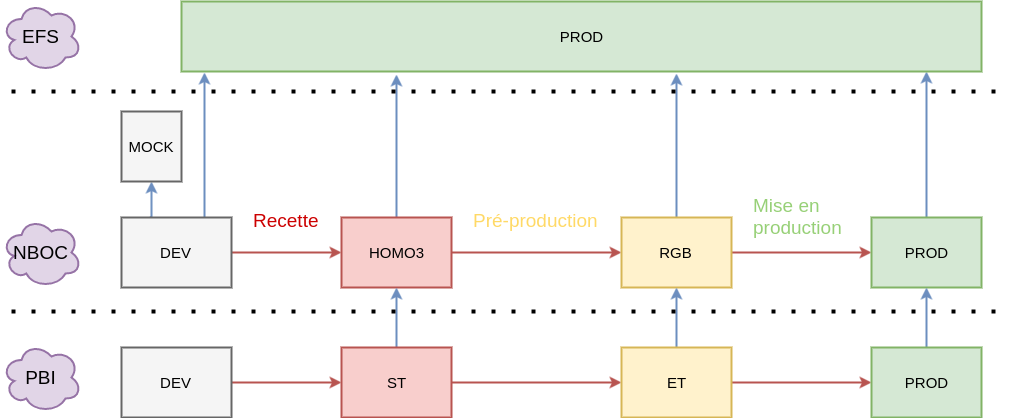
\includegraphics[scale=0.5]{images/travailNeuflizeOBC/testsFonc/environnement.png}
	\center
	\caption{Environnements}
	\label{environnement}
\end{figure}

	Ainsi, j'ai été chargé de mettre en place une procédure pouvant répondre à ce besoin. Cette dernière devait :	
	\begin{itemize}
		\item définir les cas de tests
		\item fournir des rapports d'exécution de tests détaillés
		\item nécessiter peu de développement, il était en effet inutile de réinventer la roue
		\item être gratuite
		\item être accessible à tout moment à n'importe quel membre de l'équipe de développement qui pourrait être amené à effectuer une livraison \\
	\end{itemize}